\onehalfspacing
\section{Grundlagen Softwareentwicklung und Verifikation}
Dieses Kapitel beschreibt die Grundlagen aus softwaretechnischer Sicht. Da sich die Arbeit mit dem Thema Softwaretests, sowie Testautomatisierung beschäftigt, stellt dieser Themenbereich einen großen Teil der Grundlagen dar. Zu Beginn wird auf Grundlagen zur Entwicklung bzw. Architektur von Software eingegangen. Es werden die verschiedenen Teststufen nach dem V-Modell beschrieben und erläutert. Im Anschluss werden die Grundlagen des automatisierten Testens, sowie das SICK eigene Automated Testing @ GBC07 Projekt näher erläutert.
\subsection{Software Entwicklung} 
Der Softwareentwicklungsprozess ist ein komplexer Vorgang welcher bei jedem größeren Softwareprojekt durchlaufen wird. Er dient dazu die Entwicklung einer Software klar zu strukturieren.\cite{Prof.Dr.WolfgangSchramm.2020} Heute gibt es eine Vielzahl verschiedener Vorgehensmodelle zur Softwareentwicklung, zum Beispiel Kanban, Wasserfallmodell, RUP etc., welche alle verschiedene Ansätze verfolgen. Eines der ältesten, jedoch noch gebräuchlichen Modelle, ist das V-Modell.
Das V-Modell beschreibt die fünf Phasen des Entwicklungsprozesses in absteigender Reihenfolge:\cite{Spillner.2011}
\begin{itemize}
	\item Anforderungsanalyse
	\item Systementwurf
	\item Architekturentwurf
	\item Modulentwurf
	\item Codierung
\end{itemize}
\subsubsection{Anforderungsanalyse}
Im Rahmen der Anforderungsanalyse werden die Leistungsanforderungen an das Softwareprojekt ermittelt. Hierzu ist ein enger Kontakt zum Auftraggeber notwendig. Man unterscheidet zwei Kategorien von Anforderungen:
\begin{itemize}
	\item Funktionale
	\item Nicht Funktionale
\end{itemize}
Funktionale Anforderungen beschreiben Funktionen, welche das System konkret anbieten muss, zum Beispiel addieren und subtrahieren bei der Entwicklung eines Taschenrechners. Nicht funktionale Anforderungen sind zum Beispiel das Erfüllen einer Coding-Guideline, oder die universelle Verwendbarkeit einer Software. Die nicht funktionalen Anforderungen lassen sich weiterhin in Prozess und Qualitätsanforderungen unterteilen.\cite{Broy.2021}. Das Ergebnis der Anforderungsanalyse ist ein Pflichtenheft (\ac{SRS}, welches im Anschluss als Grundlage für die Entwicklung der Software und weiterhin auch bei der  Endabnahme durch Kunden dient.
\subsubsection{Systementwurf}
Der Systementwurf im V-Modell ist die Beschreibung des prinzipiellen Aufbaus und der querschnittlichen Eigenschaften des zu entwickelnden Systems, ohne hierbei auf die Funktionsweise einzelner Systemelemente im Detail einzugehen\cite{ITBeauftragterderBundesregierung.2005}. Hierbei wird die grobe Architektur des Systems entwickelt und zum Beispiel auch die Verteilung von Servern und Clients berücksichtigt.
\subsubsection{Architekturentwurf}
Die Architektur der Software ist die Grundlage jedes Programms. Durch sie werden die einzelnen Komponenten, sowie deren Schnittstellen zueinander beschrieben.
\begin{quote} \dq Die grundlegende Organisation eines Systems, dargestellt durch dessen Komponenten, deren Beziehungen zueinander und zur Umgebung sowie den Prinzipien, die den Entwurf und die Evolution des Systems bestimmen.\dq~ ~\cite{WilhelmHasselbring.2006}\end{quote} Im Unterschied zum Systementwurf liegt hierbei der Fokus rein auf den verschiedene Softwarekomponenten.
Bei der Entwicklung einer Architektur sollten die Prinzipien der Softwareentwicklung wie zum Beispiel KISS, Kopplung und Kohäsion, Seperation of Concerns etc. beachtet und angewendet werden.\cite{Broy.2021}. Die Architektur hat einen großen Bestandteil daran, die Software skalierbar, persistent und effizient zu gestalten.
 Für die Entwicklung einer konkreten Architektur stehen verschiedene Architekturmuster zur Verfügung. Schichtenarchitekturen, Pipe-Filter Modelle, das MVC Design und das Plugin-Architekturmuster sind nur einige Beispiele.
\subsubsection*{Schichtenarchitekturen}
Eine der am häufigsten verwendeten Architekturen ist das Schichtenmodell.\cite{Prof.Dr.WolfgangSchramm.2009} Hierbei wird das System in verschiedene Schichten eingeteilt. Die einzelnen Schichten bauen aufeinander auf, sodass eine höhere Schicht auf die niedrigeren zugreifen kann, jedoch nicht auf die Schichten über ihr. Bei einer strikten Schichtenarchitektur darf darüber hinaus nur auf die direkt darunter liegende Schicht zugegriffen werden. Man unterscheidet bei dieser Art der Architektur verschiedene Modelle, so kommen zum Beispiel zwei-Schicht, drei-Schicht usw. Modelle zum Einsatz. Bei einer zwei-Schicht Architektur wird das Projekt im Allgemeinen in eine Anwendungs- und eine Datenerhaltungsschicht gegliedert. Bei einer drei-Schicht wird die Anwendungsschicht in eine Dialog- (Benutzeroberfläche) und eine Fachkonzeptschicht aufgeteilt. Je mehr Schichten zur Architektur hinzugefügt werden, desto feiner kann die Software gegliedert werden.\cite{Prof.Dr.WolfgangSchramm.2009} Besonders bekannt sind Schichtenarchitekturen aus der Netzwerktechnik. Das ISO/OSI Modell ist eine sieben-Schichten Architektur. 
\subsubsection{Modulentwurf}
Nachdem die konkrete Softwarearchitektur entwickelt wurde, liegt der Fokus in diesem Schritt darauf die Software in einzelne Teile zu zerlegen und diese der Architektur entsprechend, aufzubauen. Einzelne Softwarebestandteile, welche sich eigenständig Kapseln lassen, werden als Module bezeichnet. Die verschiedenen Module haben Schnittstellen durch welche auf ihre Funktionalität zugegriffen werden kann. Die umsichtige Klassifikation in Komponenten ist von großer Bedeutung, da diese gerade in Bezug auf die Wiederverwendbarkeit der Komponenten für andere Softwareprojekte eine große Rolle spielt. Eine Möglichkeit der Darstellung  verschiedener Module ist zum Beispiel die Form des Klassendiagramms.
\subsection{Warum Software Tests?}
Bei der professionellen Softwareentwicklung sind Softwaretests heute unabdingbar. Fehler in Software haben besonders in den letzten Jahren vermehrt dramatische Folgen gehabt. Der Absturz mehrerer Boeing 787 Max, für welchen wohl Softwareprobleme die Ursache waren \cite{tagesschau.2021} ist nur ein Beispiel aus vielen. Aber auch wenn Softwarefehler nicht solch katastrophale Folgen haben können sie hohe Kosten verursachen. 
Werden Fehler frühzeitig entdeckt und behoben, lassen sich diese Probleme abmildern. Die Kosten eines Fehlers steigen mit der Zeit seiner Existenz.\cite{DanielLindner.2020}
Um die Folgen fehlerhafter Software abzumildern spielt das Testen von Software in heutigen Entwicklungsprozessen eine zentrale Rolle. Als Leitlinie für das Durchführen und Planen von Softwaretests stehen verschiedenen Normen zur Verfügung. Als wegweisende Norm f{\"u}r Software-Systemtests wird der IEEE Standard 829 (Test Documentation) gesehen. Dieser wurde bereits 1983 eingef{\"u}hrt und in der zwischen Zeit mehrfach {\"u}berarbeitet. Der Standard beschreibt den Systemtestprozess und die Testdokumentation.~\cite[S.~21]{Witte.2016} Weiterhin werden Softwaretests im ISO-Standard 9126 sowie IEC-29119 behandelt. Der Testprozess wird nach IEEE 829 in sieben Schritte eingeteilt:
\begin{itemize}
	\item Testplanung
	\item Testfallspezifikation
	\item Testentwurf
	\item Testdarstellung (Ist und Soll)
	\item Testausführung
	\item Testauswertung
	\item Testabnahme
\end{itemize}
Der ISO-Standard 9126 hingegen befasst sich eher mit Softwarequalität im Allgemeinen. In der Norm ist definiert was für die Messung der Softwarequalität erforderlich ist. Im ISO Standard IEC-29119 hingegen ist der Testbegriff, Dokumentation, Testprozess, sowie die einzelnen Testtechniken definiert. Hier ist zum Beispiel der Begriff sowie der Aufbau von Unit Tests definiert.\cite{Witte.2016}
Aufgrund der zentralen Rolle von Softwaretests verfolgen einige Entwickler das Konzept des Testdriven Development, welches vorsieht den produktiv Code auf Grundlage der zuvor erstellten Tests zu entwickeln.
	\subsection{Arten von Softwaretests}
	In der modernen Softwareentwicklung wird zwischen verschiedenen Arten von Software Tests unterschieden. Die Einteilung gestaltet sich schwierig, da eine große Vielfalt an verschiedenen Begriffen bzw. Bezeichnungen besteht\cite{DanielLindner.2020}:
\begin{itemize}
	\item Abnahmetests
	\item Systemtests
	\item Integrationstests
	\item Modultests (Unit Tests)
\end{itemize}
Das \dq \nameref{fig:V-Model.jpg}\dq~zeigt die Entwicklungsphasen und die entsprechenden Testphasen in hierarchischer Ordnung auf.
\begin{figure}[h]
  \centering
   \includegraphics[width=1\textwidth]{img/V-Model.jpg} 
   \caption[V-Model]{ V-Model \cite{Witte.2016}}
   \label{fig:V-Model.jpg}
\end{figure}
\newpage
\subsubsection{Modultests}
Als Modultests oder auch Unit Tests werden Tests beschrieben, welche das Design einer Softwarekomponente testen. Der Test läuft also gegen die Funktionalität der Komponente selbst. Man versucht dabei, die kleinste Sinnvolle Einheit zu überprüfen \cite{Grunfelder.2017}. Unit  Tests sind ein dynamisches Testverfahren. Meist werden sie als erste Tests nach dem Schreiben des Codes angewendet. Das Prinzip des Unit-Testing beruht darauf, dass Software aus einzelnen Modulen besteht, welche zu einem gesamten Programm zusammengesetzt werden. Durch Unit Tests werden diese einzelnen Module (Komponenten) isoliert getestet und geprüft, ob jede Komponente für sich korrekt arbeitet. Ein Beispiel wäre zum Beispiel das Abprüfen eines Umrechnungstools für Einheiten in einer Kalorienzähler App. Ein beispielhafter Unit Test ist in Abbildung \dq \nameref{fig:UnitTest_Einfach.jpg}\dq~dargestellt.\newpage
\begin{figure}[h]
  \centering
   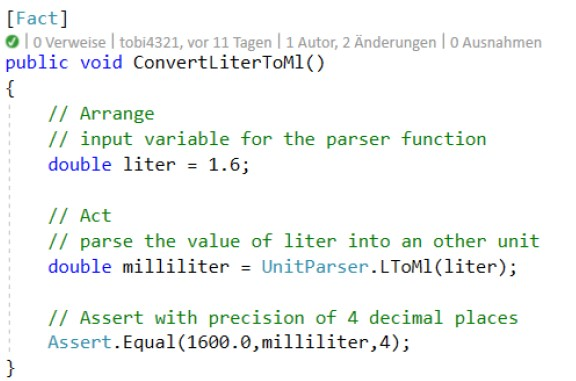
\includegraphics[width=0.75\textwidth]{img/UnitTest_Einfach.jpg} 
   \caption[Einfacher Unit Test]{ Einfacher Unit Test \cite{MarvinBock.2021}}
   \label{fig:UnitTest_Einfach.jpg}
\end{figure}
Bei einem Unit Test sollte zuerst die Funktion der Komponente geprüft werden. Im  Falle eines Umrechnungstools wären hier zum Beispiel Tests mit erwarteten Daten zielführend. Nachdem die Grundfunktionalität getestet ist, sollten die Grenzfälle betrachtet und Fehlerfälle eingebaut werden. Grenzfälle können zum Beispiel Werte am Rand des definierten Wertebereiches der Funktion sein. Fehlerfälle können zum Beispiel die Eingabe eines negativen Wertes statt eines erwarteten positiven, oder die Verwendung von Werten außerhalb des Wertebereichs sein. In der Regel wird für jede Teilkomponente ein eigener Unit Test erstellt, welcher die Funktion dieser Teilkomponente unabhängig von den anderen Komponenten betrachtet. In der Realität lassen sich jedoch die Komponenten oft nur schwer von einander Abgrenzen. Ein Beispiel hierfür ist der Aufruf einer anderen Komponente und das Verarbeiten des Rückgabewertes. Bei der Implementierung muss der Aufruf der Unterfunktion bzw. deren Rückgabewert simuliert werden, um daraus resultierende Fehlerfälle auszuschließen bzw. mit Absicht herbeizuführen. Die Simulation einer Unterkomponente wird auch als Stub bzw. Mock bezeichnet.\cite{Grunfelder.2017}
Für die Entwicklung und Durchführung von Unit Tests wird meist ein unterstützendes Testframeworke verwendet. Beispiele für Testframeworkes sind u.a. JUnit, TestNG oder Spock.\newpage
Bei der Erstellung kann die AAA-Normalform herangezogen werden, diese definiert die drei Hauotkomponenten jedes Unit Tests\cite{DanielLindner.2020}:
\begin{itemize}
	\item Arrange -> Initialisieren der Test-"Welt"
	\item Act -> Ausführen der zu testenden Aktion
	\item Assert -> Prüfen der Test-Zusicherung
\end{itemize}
Die ATRIP Regeln gelten als Grundlage für die Erstellung qualitativ guter Unit Tests\cite{DanielLindner.2020}:
\begin{itemize}
	\item Automatic
	\item Thorough
	\item Repeatable
	\item Independent
	\item Professional
\end{itemize}
Unit Tests sollten automatisch ablaufen (Automatic), sie sollten gründlich sowie wiederholbar sein (Thorough \& Repeatable). Weiterhin sollten keine Abhängigkeiten zwischen den einzelnen Tests bestehen (Independent) und die einzelnen Tests sollten mit Sorgfalt erstellt worden sein (Professional).
Die Testabdeckung kann nach verschiedenen Methoden ermittelt werden. Zu den gängigen Methoden zählen unter anderem die Line Coverage und die Branch Coverage. Bei der Line Covergage wird lediglich gemessen, wie viele Codezeilen mittels Tests durchlaufen werden. Bei der Branch Coverage wird geprüft, ob der Test alle Verzweigungen zum Beispiel bei einem if Statement mindestens einmal durchlaufen hat.\cite{Grunfelder.2017}
Je nach Art und Umfang des Programmes kann es sehr aufwendig sein jede Komponente einer Software mit Unit Tests abzudecken. Dennoch ist eine Testabeckung von über 80\% anzustreben. Bei der Erstellung von Tests sollt jedoch stets das Optimum zwischen Aufwand und Kosten gefunden werden.\cite{DanielLindner.2020}
\newpage
\subsubsection{Integrationstests}
Bei einem Integrationstest wird im Gegensatz zu Unit Tests nicht eine einzige Komponente getestet, sondern das Zusammenspiel mehrerer Komponenten. Dies bedeutet, dass in der Regel bereits verschiedenen Unit Tests von den Komponenten durchlaufen wurden. Somit kann davon ausgegangen werden, dass die Komponenten für sich isoliert fehlerfrei funktionieren. Ziel der Integrationstests ist es Fehler aufzudecken, welche das Zusammenspiel verschiedener Komponenten betreffen. Mithilfe eines Integrationstests lassen sich zum Beispiel inkompatible Schnittstellenformate oder Timing Probleme bei der Übergabe von Daten aufdecken \cite{Witte.2016}. Es wird zwischen verschiedenen Integrationsteststrategien unterschieden. Bei der Bottom-Up Methode (\dq \nameref{fig:Bottom_UP.jpg}\dq) erfolgen die Tests in umgekehrter Richtung zur Benutzer Beziehung, also von  innen nach außen. Durch dieses Vorgehen spart man sich das Erstellen der Testrümpfe, da nur die Testtreiber programmiert werden müssen.
\begin{figure}[h]
  \centering
   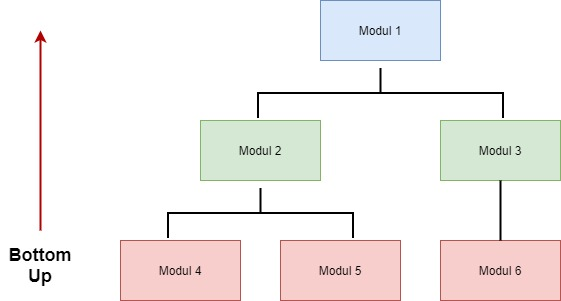
\includegraphics[width=0.70\textwidth]{img/Bottom_UP.jpg} 
   \caption{ Ablauf Bottom-Up Test}
   \label{fig:Bottom_UP.jpg}
\end{figure}
 Ein Nachteil hierbei ist, dass Fehler in der obersten Schicht erst sehr spät erkannt werden. Im Gegensatz dazu wird bei der Top-Down Methode in Richtung der Benutzer Beziehung getestet. Für diese Strategie werden zwar Testrümpfe benötigt, jedoch werden Fehler in der obersten Schicht früher erkannt. Eine weitere Möglichkeit ist der Urknalltest, hierbei werden alle Komponenten getrennt entwickelt und in einem Schritt integriert. Dieses Vorgehen erschwert allerdings die Fehlersuche. Neben diesen drei Methoden kommt auch eine Hybride Mischung aus Bottom-Up bzw. Top-Down zum Einsatz.  
\subsubsection{Systemtests}
Systemtests sind Tests welche das gesamte System gegen dessen Anforderungen testen. Üblicherweise wird als Testumgebung ein Abbild der späteren Produktivumgebung gewählt und der Test mit entsprechenden Testdaten (zum Beispiel Datenbankeinträgen, etc.) durchgeführt. Wichtig hierbei ist, dass ein Abbild der Produktivumgebung geschaffen wird und diese nicht selbst zu verwenden. Unter Umständen kann es sonst zu Schäden bzw. Ausfällen an der Produktivumgebung kommen. Weiterhin sind die Test dadurch aber auch schwer reproduzierbar. Bei einem Systemtest werden sowohl funktionale als auch nicht funktionale Qualitätsmerkmale der Software getestet\cite{Witte.2016}. Hierzu wird zwischen funktionalen und nicht funktionalen Tests unterschieden. Funktionale Tests prüfen, ob die Software, die in der Spezifikation geforderten Funktionen bereitstellt. Nicht funktionale Tests prüfen Zuverlässigkeit, Benutzbarkeit, Effizienz, Veränderbarkeit und Übertragbarkeit. In Abbildung \dq \nameref{fig:Systemtest.jpg}\dq~wird ein Überblick über mögliche Systemtests dargestellt.\newline
\begin{figure}[h]
	\centering
  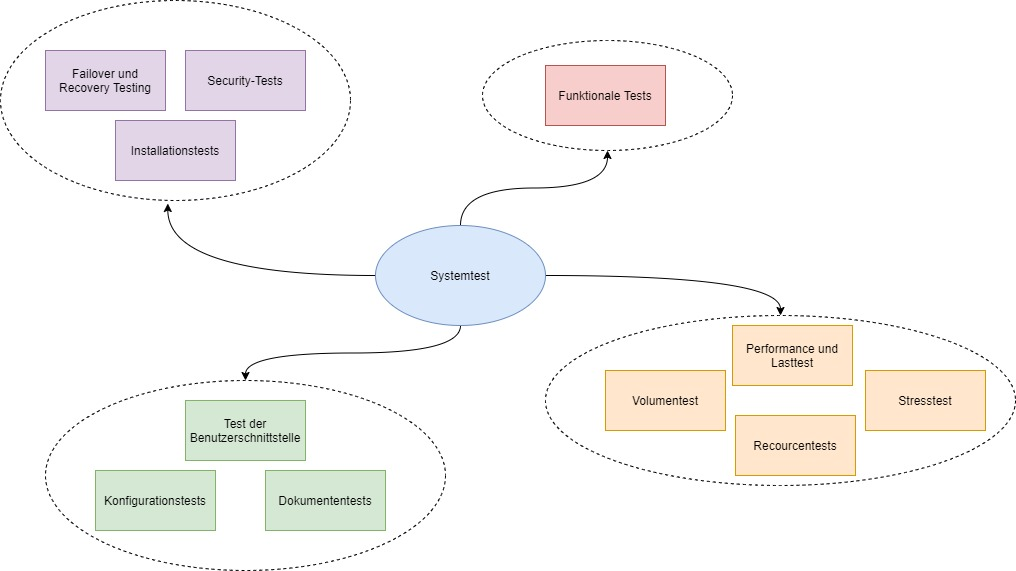
\includegraphics[width=1\textwidth]{img/Systemtest.jpg} 
   \caption{Systemtest}
  \label{fig:Systemtest.jpg}
\end{figure}
\cleardoublepage
Systemtests gelten als der wichtigste Testschritt: \begin{quote}\dq Systemtests sind die wichtigste Teststufe. In Systemtests werden Designfehler,Inkompatibilitäten zur Hardware, zeitabhängige Fehler und zum Teil auch Lücken in der Spezifikation gefunden.\dq~ ~\cite[S.~195]{Grunfelder.2017}\end{quote} Systemtests können aufgrund der breiten Testabdeckung sehr umfangreich und aufwendig sein. Eine Automatisierung der Tests macht jedoch nur Sinn, wenn die Tests mehrfach wiederholt werden sollen, da die Implementierung automatischer Tests einen etwa zehnfach höheren Aufwand bedeutet\cite{Basler.2016}. Die Messung der Testabdeckung lässt sich bei Systemtests ebenfalls nur schwer realisieren. \cite{Grunfelder.2017}

\subsubsection{Abnahmetests}
Im Gegensatz zu den bisher behandelten Teststufen wird der Abnahmetest meist nicht vom Hersteller, sondern direkt vom Kunden durchgeführt. Der Test hat nicht das Ziel eventuelle Fehler aufzudecken, sondern das Vertrauen des Kunden in das Produkt bestärken. Der Abnahmetest ist hierbei fester Bestandteil des Vertrags zwischen Kunde und Lieferant, sowie ein Meilenstein in der Projektplanung.\newline Durch einen erfolgreichen Abnahmetest werden verschiedene Ereignisse, wie zum Beispiel Zahlungsfristen oder Garantievereinbarungen getriggert. Um Probleme während des Abnahmetests zu verhindern sollten die Rahmenbedingungen (Test Umgebung und Anforderungen an den Test) im Vorhinein Vertraglich geregelt sein. Um repräsentative Ergebnisse zu erhalten kann es auch angebracht sein, den Abnahme- bzw. Akzeptanztest mit verschiedenen Benutzergruppen durchzuführen.\cite{Witte.2016}
\newpage
\subsection{Testsuite}
Als Testsuite wird eine Zusammenstellung mehrerer Testf{\"a}lle f{\"u}r den Test einer Komponente oder eines System bezeichnet, bei der die Nachbedingungen des einen Tests als Vorbedingungen des folgenden Tests genutzt werden sollen.~\cite{ISTQBGlossary.2021} Durch die Verwendung einer Testsuite lassen sich Software Tests einfacher automatisieren und wiederverwenden. Durch den Einsatz von Testsuites lassen sich die Testfälle aus dem Testplan besser clustern. Ein möglicher Aufbau eines Testkonzepts ist in Abbildung \dq \nameref{fig:Testsuite.jpg}\dq~schematisch dargestellt.
\begin{figure}[h]
	\centering
  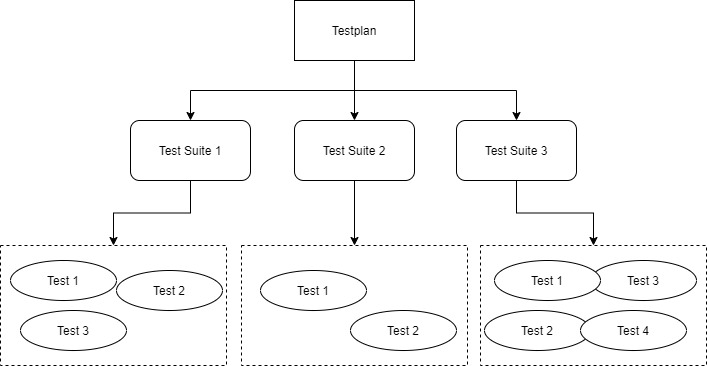
\includegraphics[width=1\textwidth]{img/Testsuite.jpg} 
   \caption{Testsuite}
  \label{fig:Testsuite.jpg}
\end{figure}
\newpage
	\subsection{Testautomation}
	Im Rahmen der Softwareentwicklung sollten Softwartests schon frühzeitig in den Entwicklungsprozess eingebunden werden. Das Konzept einer CI Pipeline, wie es heute in vielen Entwicklerteams zum Einsatz kommt, sieht Softwaretests als klaren Bestandteil des Entwicklungsprozess an. Eine CI Pipeline ist in Abbildung \dq \nameref{fig:CICD.jpg}\dq~zu sehen.
\begin{figure}[h]
	\centering
  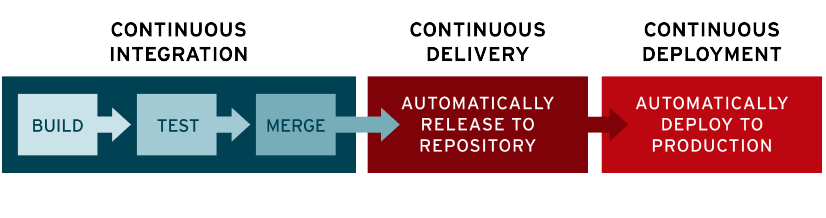
\includegraphics[width=1\textwidth]{img/CI.png} 
   \caption[CI/CD Prozessablauf]{CI/CD Prozessablauf \cite{RedHat.2021}}
  \label{fig:CICD.jpg}
\end{figure}

Bei einer strikten Umsetzung des CI Prozesses befindet sich im Repository nur getesteter Code\cite{RedHat.2021}. Zur Vereinfachung dieses Prozesses werden die Testvorgänge automatisiert. Durch die Automatisierung von Tests wird sowohl die Reproduzierbarkeit gesteigert, als auch die Testabdeckung erhöht. Weiterhin werden durch automatisierte Tests Kosten und Zeit gespart\cite{Witte.2016}. Jedoch ergeben sich durch automatisiertes Testen auch Nachteile. So können Testergebnisse nicht schon während der Testdurchführung interpretiert werden. Außerdem ist der Aufwand für die Implementierung höher als bei manuellen Test\cite{Witte.2016}. Bei der Automatisierung von Tests geht es vorwiegend um die automatische Ausführung und weniger um die maschinelle Erstellung von Tests. Hierfür stehen eine Vielzahl von verschiedenen Tools zur Verfügung. Im Kapitel \dq\nameref{sec:Automated_Testing}\dq~wird das bei SICK STEGMANN verwendete Tool näher erklärt.
\newpage

\subsection{Projekt Automated Testing @ GBC07}\label{sec:Automated_Testing}
Das Projekt Automated Testing @ GBC07 ist ein Projekt, welches bereits seit mehren Jahren durch die Abteilung Research and Development der SICK STEGMANN GmbH vorangetrieben wird. Ziel des Projektes ist es, die Testprozesse im Unternehmen auch über verschiedene Abteilungen hinweg zu vereinfachen und gemeinsame Standards zu definieren. Das Projekt umfasst die gesamte Testumgebung sowohl im Software als auch Hardware Bereich. Der grundsätzliche Aufbau des Projekts ist in der Abbildung \dq \nameref{fig:autotest.jpg}\dq~dargestellt.
Zu erkennen ist, dass der komplette Testablauf automatisiert wurde. Durch den Aufbau des Projekts lassen sich die verschiedene Testarten vom Unit Test bis hin zum Systemtest durchführen. Für den Standardentwickler ist der Testaufwand so deutlich geringer. Er hat die Möglichkeit die entsprechenden Tests in einem Einheitlichen Frameworke zu Entwicklern und auch Tests von anderen Projekten bzw. Entwicklern wiederzuverwenden. Die Tests werden in der SICK eigenen Programmiersprache ITE oder in Python geschrieben. ITE ist an C++ angelehnt, wurde jedoch an einigen Stellen speziell auf die Bedürfnisse des SICK Konzerns angepasst. Herzstück des Testsystems ist der Test Automation Slave. Dieser enthält alle Komponenten, welche zur Konfiguration und Ausführung der Tests benötigt werden. Das Modul Access and Test Creation dient zur Konfiguration des Testablaufs. Die Persistenzschicht dient zur Ablage der erstellten Testpläne. Der Test Controller dient im Anschluss zur Ausführung der Testpläne. Das Modul Test Cases enthält die konkreten Testfälle auf welche der Test Controller je nach Anforderung des Testplans zurück greift.\cite{SICKAG.04.2021}
\begin{figure}[h]
	\centering
  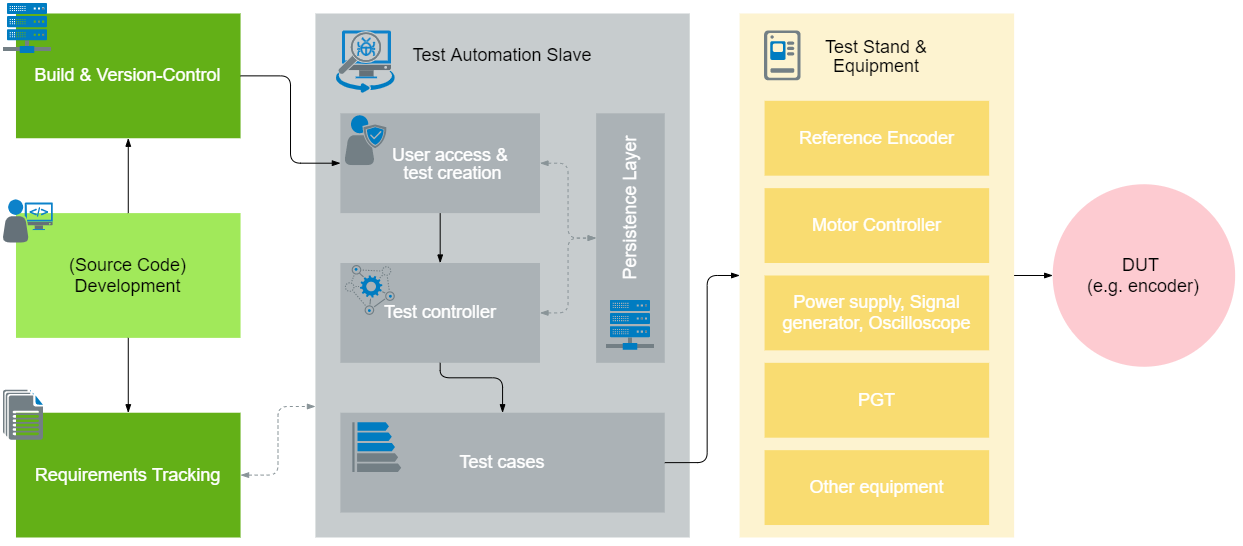
\includegraphics[width=1.25\textwidth, angle=90]{img/automated_testing.png} 
   \caption[Aufbau Automated Testing @ GBC07]{Aufbau Automated Testing @ GBC07 \cite{SICKAG.04.2021}}
  \label{fig:autotest.jpg}
\end{figure}

\cleardoublepage





\newpage
\section{Technische Grundlagen}
Im Kapitel Technische Grundlagen werden die Hardware Grundlagen wie zum Beispiel Aufbau und Funktionsweise eines Drehgebers oder die Funktionsweise des Hiperface Protokolls beschrieben. Durch dieses Kapitel soll ein Grundwissen über die verwendete Hardware geschaffen werden, welches für das Verständnis der folgenden Konzeptionierung, sowie verschiedener Designentscheidungen notwendig ist.
\subsection{Encoder/MFB}
Encoder und Motor-Feedback-Systeme dienen klassischerweise zur Messung rotatorischer Bewegungen. Sie wandeln hierbei die Winkel zweier sich relativ zueinander drehender Objekte in ein elektrisches Signal um. \ac{MFB} und Encoder unterscheiden sich hierbei vorwiegend in ihren Einsatzgebieten. \ac{MFB} werden üblicherweise in Elektromotoren eingesetzt, wohingegen das Einsatzgebiet von Encodern breiter gefasst ist. Ein Encoder wir hierbei als Lastgeber (misst an der Lastachse), ein \ac{MFB} als Motorgeber bezeichnet.\cite[S.1]{Basler.2016}
Der technische Aufbau der Systeme ist im Grundsatz gleich, er gliedert sich in folgende drei wesentliche Bestandteile:
\begin{itemize}
	\item Sender
	\item Modulator
	\item Empfänger
\end{itemize}
Drehgeber messen die Drehbewegung einer rotativen Achse in Bezug zu einem Referenzpunkt, d.h. den Winkel zwischen der Aktuellen Position und dem Referenzpunkt.
  \begin{figure}[h]
        \centering
        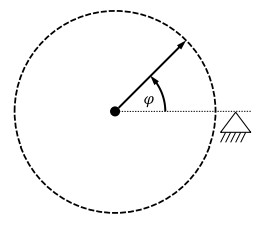
\includegraphics[width=0.5\textwidth]{img/Winkel_bei_rot_Bewegung.jpg} 
        \caption[Winkel bei rotatorischer Bewegung]{Winkel bei rotatorischer Bewegung\cite{Basler.2016}}
        \label{fig:Winkel_bei_rot_Bewegung.jpg}
    \end{figure}
Die Abbildung \dq \nameref{fig:Winkel_bei_rot_Bewegung.jpg}\dq~stellt einen Einheitskreis mit einem Radius von eins dar, in welchem sich ein Zeiger entsprechend der Rotation des Motors bewegt. Die x und y-Komponente des Zeigers können wiederum als Sinus- bzw. Cosinus-Werte dargestellt werden. Dies ist in Abbildung \dq \nameref{fig:einheitskreis_sin_cos.jpg}\dq~abgebildet.
  \begin{figure}[h]
        \centering
        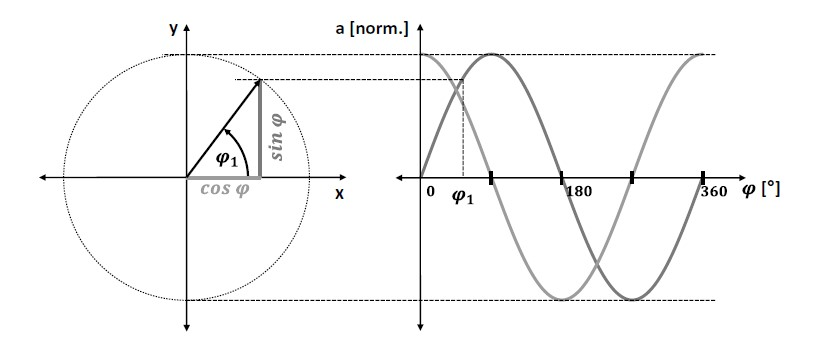
\includegraphics[width=1\textwidth]{img/einheitskreis_sin_cos.jpg} 
        \caption[Sinus- und Cosinus Darstellung beim Einheitskreis]{Sinus- und Cosinus Darstellung beim Einheitskreis \cite{Basler.2016}}
        \label{fig:einheitskreis_sin_cos.jpg}
    \end{figure}
 Durch diese Betrachtung lässt sich der Winkel zwischen Ausgangsposition und aktueller Position mittels Trigonometrischer Funktionen berechnen (Goniometrie). Die Formel lautet dementsprechend:\cite{Basler.2016}
        \begin{align*}
             \varphi = arctan \left( \frac{a_{sin}}{a_{cos}} \right)
			\label{Test}        
        \end{align*}
Um eine höhere Auflösung zu erreichen, wird in der Praxis eine Umdrehung nicht als eine Sinus bzw. Cosinus dargestellt, sondern der Vollwinkel in mehrere Teilwinkel unterteilt. Diese werden dann wiederum durch eine Sinus- bzw. Cosinus-Periode repräsentiert. 
Ein Drehgeber liefert demnach als Ausgangssignal Sinus bzw. Cosinus Werte, aus welchen sich die aktuelle Lage der Welle berechnen lässt.
Im Bereich der Drehgeber gibt es eine Vielzahl verschiedener Ansätze zur Bestimmung dieses Winkels, bzw. der aktuellen Position des Zeigers.
Eine Klassifizierung ist zum Beispiel anhand des sensorischen Messprinzips möglich. Hierbei wird zwischen optisch, magnetisch, induktiv, kapazitiv und resistiv potentiometrisch unterschieden.
Da sich diese Arbeit konkret mit dem SKS bzw. SKM beschäftigt, welcher als optischer Drehgeber realisiert ist, wird im Verlauf lediglich auf optische Drehgeber eingegangen.

Der grundsätzliche Aufbau optischer Drehgeber setzt sich aus einer Codescheibe (Modulator), einer Sende- Empfangseinheit sowie einer Leiterplatte zusammen. Die Leiterplatte nimmt die Signale der Sende- Empfangseinheit auf und verarbeitet diese, darüber hinaus stellt sie eine Kommunikationsschnittstelle zur Verfügung. Die einzelnen Komponenten sowie ihr 			Zusammenspiel sind in Abbildung \dq \nameref{fig:Schematischer_aufbau_encoder.jpg}\dq~dargestellt.\newline
  	\begin{figure}[h]
        \centering
        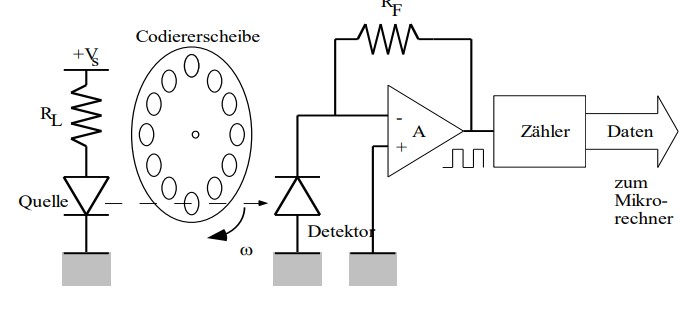
\includegraphics[width=1\textwidth]{img/Schematischer_aufbau_encoder.jpg} 
        \caption[Komponenten eines MFB]{Komponenten eines \ac{MFB} \cite{Dr.MartinDo.11.11.2020}}
        \label{fig:Schematischer_aufbau_encoder.jpg}
    \end{figure}
    
Der Sender bzw. Empfänger sind fest montiert, die Codescheibe ist beweglich. Die Codescheibe ist mit der Welle verbunden und dreht sich somit äquivalent zu dieser. Durch die Codescheibe wird der vom Sender ausgesendete Lichtstrom moduliert.  Die Modulation erfolgt durch den Aufbau der Codescheibe mittels lichtdurchlässiger und undurchlässiger Felder. Der modulierte Lichtstrom (Hell-Dunkel-Muster) fällt auf den Empfänger. Durch diesen wird die optische Energie in elektrische gewandelt. Das hier erläuterte Verfahren wird als Schattenbildverfahren bezeichnet. Daneben kommen  auch andere Verfahren, wie das Basis diffraktive (basierend auf optischer Beugung), oder Verfahren basierend auf dem Morie-Effekt zum Einsatz.
Bei der Modulation des Lichtstrom ist die Bauart der Codescheibe bzw. deren Codierung maßgeblich. Man unterscheidet hierbei zwischen inkrementellen und absoluten Codierungen. Bei der inkrementellen Codierung wird nicht die absolute Winkelinformation, sondern lediglich eine Winkeländerung ausgegeben. Eine inkrementelle Codescheibe ist meist durch regelmäßige, trapezförmige Bereiche, welche abwechselnd lichtdurchlässig bzw. -undurchlässig sind realisiert. So lässt sich ein Sinus- bzw. Rechtecksignal erzeugen. Bei inkrementellen Drehgebern ist eine Referenzfahrt im Startvorgang des Drehgebers notwendig. Bei absoluten Drehgebern kann jederzeit die absolute Winkelposition ermittelt werden. Der Aufbau der Codescheibe gliedert sich hier in zwei Bestandteile, eine inkrementelle Codespur, sowie weitere Signalspuren, welche gemeinsam einen Code (zum Beispiel binär-, Gray-, oder Pseudo-Random-Code)ergeben. Durch diesen Aufbau entfällt die Referenzfahrt. Ein Beispiel für unterschiedliche Codespuren ist Abbildung \dq \nameref{fig:Codescheibe.jpg}\dq. 	
\begin{figure}[h]
        \centering
        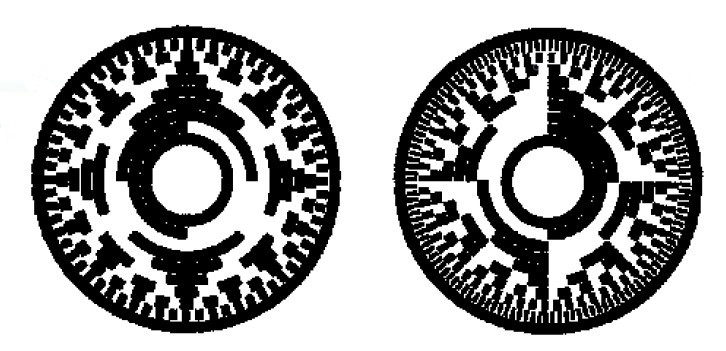
\includegraphics[width=1\textwidth]{img/Codescheiben.jpg} 
        \caption[Codescheiben, links Graycode, rechts Binär]{Codescheiben, links Graycode, rechts Binär \cite{Dr.MartinDo.11.11.2020}}
        \label{fig:Codescheibe.jpg}
    \end{figure} 

Neben der Unterscheidung zwischen inkrementell und absolut können Drehgeber auch in Single- und Multiturn Drehgeber unterteilt werden. Bei einem Singelturn Geber wird immer nur eine Umdrehung mittels der Codescheibe aufgelöst. Bei Multiturn Gebern wird die Codescheibe um ein untersetztes Getriebe ergänzt. Das Getriebe wird wie die Codescheibe durch die Welle angetrieben. Die aktuelle Position des Getriebes wird über Hall-Sensoren ermittelt. Durch diesen Aufbau wird ein Messbereich von bis zu 4096 Umdrehungen erreicht. \cite{Basler.2016} 
	In dieser Arbeit wird der SKx behandelt. Der SKS bzw. SKM ist ein durch die Firma SICK STEGAMNN entwickeltes \ac{MFB}. Der SKx ist ein absolut arbeitender Drehgeber, und bereits seit mehreren Jahren eines der meistverkauften Produkte der SICK STEGMANN GmbH. Die Bezeichnung SKS steht für die Ausführung als Singleturn Geber, SKM für Multiturn. Als Besonderheit des Gebers ist die Hiperface Schnittstelle zu erwähnen.
	\begin{figure}[h]
        \centering
        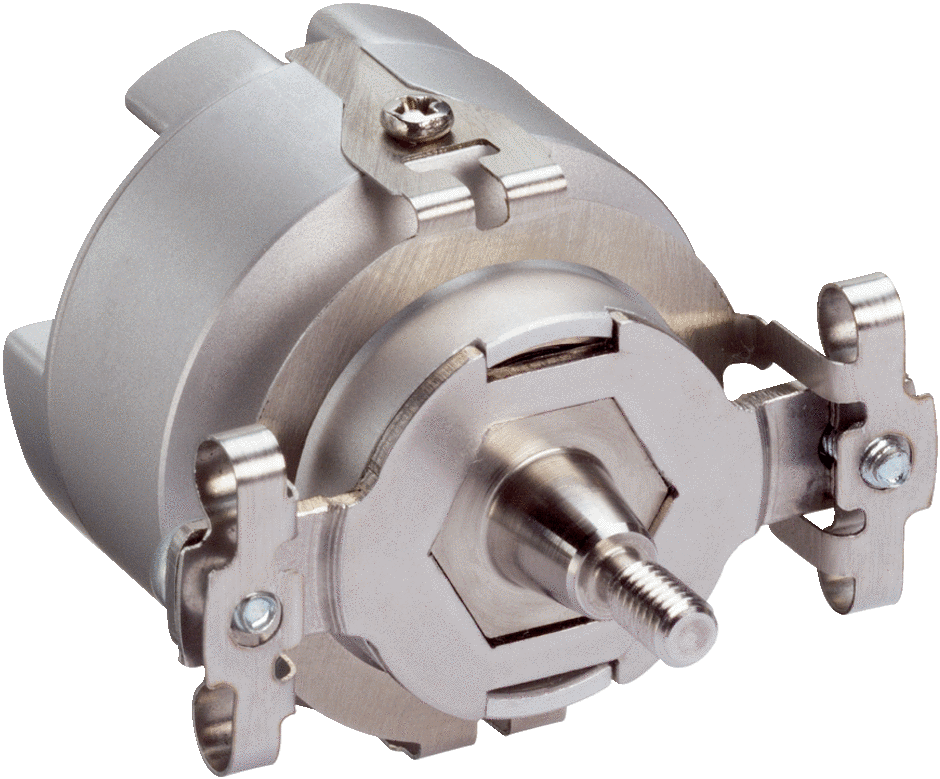
\includegraphics[width=0.5\textwidth]{img/SKM36.png} 
        \caption[SKM36]{ SKM36 \cite{SICKAG.2021}}
        \label{fig:SKM36.jpg}
    \end{figure}
    \newline
\newpage

\subsection{Hiperface Protokoll}
Das Hiperface Protokoll ist eine durch die Firma SICK entwickelte, offene Schnittstelle. Die Hiperface  Schnittstelle gilt als Standard Schnittstelle im Bereich der Motorfeedbacksysteme
Der Name Hiperface steht für High Performance Interface. Die Hiperface Schnittstelle setzt sich  aus einer busfähigen RS485 Schnittstelle (Digital) Sowie einer analogen Schnittstelle zur Übertragung der Sinus und Cosinus Signale zusammen. 
\begin{figure}[h]
  \centering
   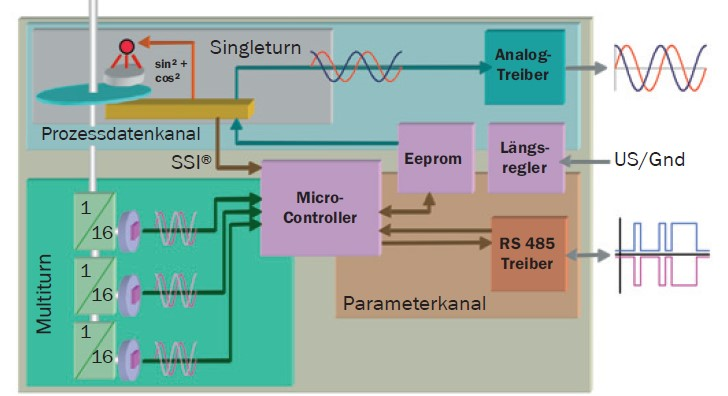
\includegraphics[width=1\textwidth]{img/Aufbau_Hiperface_MFB.jpg} 
   \caption[Aufbau Hiperface MFB]{ Aufbau Hiperface \ac{MFB} \cite{SICKAG.2021}}
   \label{fig:AufbauHiperfaceMFB.jpg}
\end{figure}
In Abbildung \dq \nameref{fig:AufbauHiperfaceMFB.jpg}\dq~ist der Aufbau eines Hiperface Gerätes schematisch dargestellt. Die Codescheibe wird bei diesem Aufbau neben der absoluten Codespur um eine Inkrementelle ergänzt.
 Zur Realisierung der Schnittstelle sind lediglich acht Leitungen zwischen \ac{MFB} und verarbeitendem System notwendig. Zwei Leitungen dienen zur Übertragung der Versorgungsspannung (7-12V), vier Leitungen werden zur Übertragung der Inkrementellen Sinus und Cosinus benötigt und die verbleibenden zwei Leitungen dienen zur Kommunikation mittels RS485 Schnittstelle. Die Kommunikation mittels der bidirektionalen RS485-Schnittstelle beginnt  jeweils mit der Angabe der Zieladresse. Darauf folgt der entsprechende Befehl. Die Nachricht endet mit einer Prüfsumme. Jede Nachricht beginnt mit einem Startbit und endet mit einem Stopbit, dazwischen befinden sich acht Datenbit. Es wird zwischen zwei Arten von Nachrichtenformaten unterschieden (Adress und Command). Bei Adress wird lediglich die Teilnehmernummer übertragen, hierfür werden fünf Bit verwendet. Die default Teilnehmernummer lautet 40h. Alle weiteren Teilnehmernummern beginnen ab 40h, was dazu führt, dass lediglich fünf Bit Variabel gestaltet sind. Wie in Abbildung \dq \nameref{fig:Teilnehmernummer.jpg}\dq~zu sehen bleibt durch die Beschneidung des Adressbereichs das Bit sieben immer  eins und das Bit sechs immer null. Lediglich die Bits 1-5 sind variabel.
 \begin{figure}[h]
  \centering
   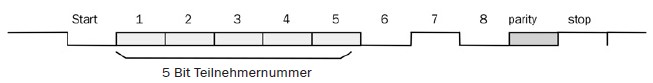
\includegraphics[width=1\textwidth]{img/Teilnehmernummer.jpg} 
   \caption[Aufbau Adresse Hiperface]{Aufbau Adresse Hiperface \cite{SICKAG.2016}}
   \label{fig:Teilnehmernummer.jpg}
\end{figure}
 Bei Command Befehlen ist das Vorgehen sehr ähnlich, hier sind jedoch sechs Bit variabel und das siebte Bit immer eins. Die einzelnen Befehle sind von 42h bis 67h codiert. Ein einfacher Befehl ist in \dq \nameref{fig:Positionlesen.jpg}\dq~zu sehen.
\begin{figure}[h]
  \centering
   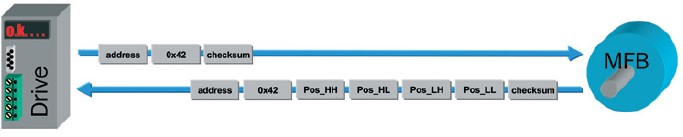
\includegraphics[width=1\textwidth]{img/Positionlesen.jpg} 
   \caption[Lesen der aktuellen Position über RS485]{ Lesen der aktuellen Position über RS485  \cite{SICKAG.2016}}
   \label{fig:Positionlesen.jpg}
\end{figure}

Neben der aktuellen Position des Gebers lassen sich über die Hiperface Schnittstelle noch weitere Informationen wie zum Beispiel der Status des Gerätes, oder das elektronische Typenschild auslesen. Weiterhin ist es ebenfalls möglich  verschiedene Register im \ac{MFB} über die Schnittstelle zu beschreiben, oder einen Reset des Gerätes durchzuführen.

\newpage

\subsection{ST7/ STM8}
Der ST7 ist ein durch die Firma STMicroelektronics vertriebener Mikrocontroller. Zur ST7 Familie gehören verschiedene Derivate, so ist zum Beispiel eine lite- oder eine automotiv Variante verfügbar. Alle Modelle der ST7 Familie gehören zu den 8 Bit Mikrocontrollern. Für den SKS bzw. SKM wird konkret der ST7234BK6T3 verwendet. Der Controller verfügt über einen integrierten A/D Wandler, Timer und  eine SPI sowie SCI Schnittstelle. Er basiert auf einer Von-Neumann-Architektur.\cite{STMicroelektronics.2008}. Der ST7 stellt das Herzstück des SKS bzw. SKM dar. Er dient hier zur Kommunikation via Hiperface und übernimmt die Berechnung der absoluten Position. Der STM8 ist die neueste acht Bit Controllerlinie von STMicroelektronics. Die STM8 Familie basiert auf auf einer modifizierten Harvard-Architektur\cite{STMicroelektronics.2017}. Neben mehr Speicherplatz  verfügt der Controller auch über deutlich mehr peripherie Möglichkeiten im Vergleich zu seinem Vorgänger. %%ggf. noch ein bisschen text ergänzen?
